\chapter{Implementação no Middleware Ginga-NCL} \label{cap:cap5}

O Ginga-NCL é o subsistema do \textit{middleware} Ginga, padrão do Sistema Brasileiro de TV Digital, que permite a execução de aplicações multimídia especificadas na linguagem NCL \cite{ABNT:2011aa}. Atualmente, o subsistema dá suporte apenas a interações de um usuário por meio do controle remoto ou mouse. Visando dar suporte a outras modalidades de interação, suporte multiusuário e armazenamento de informações contextualizadas por usuários (ou grupo de usuários) nas aplicações, esta tese propõe a inclusão de novos componentes no \textit{middleware}\footnote{A implementação de extensão do Ginga-NCL apresentada neste trabalho pode ser acessada em  bit.do/gingaMultimodalBranch.}, conforme será detalhado nas seções a seguir. %mostra a Figura \ref{fig:arquitetura}. 
Para o desenvolvimento da proposta foi utilizada a implementação de referência da máquina de apresentação\footnote{https://github.com/TeleMidia/ginga} do Ginga-NCL. A Figura \ref{fig:arquitetura} ilustra a arquitetura da implementação estendida do \textit{middleware} Ginga-NCL.

\begin{figure}[h!]
    \centering
    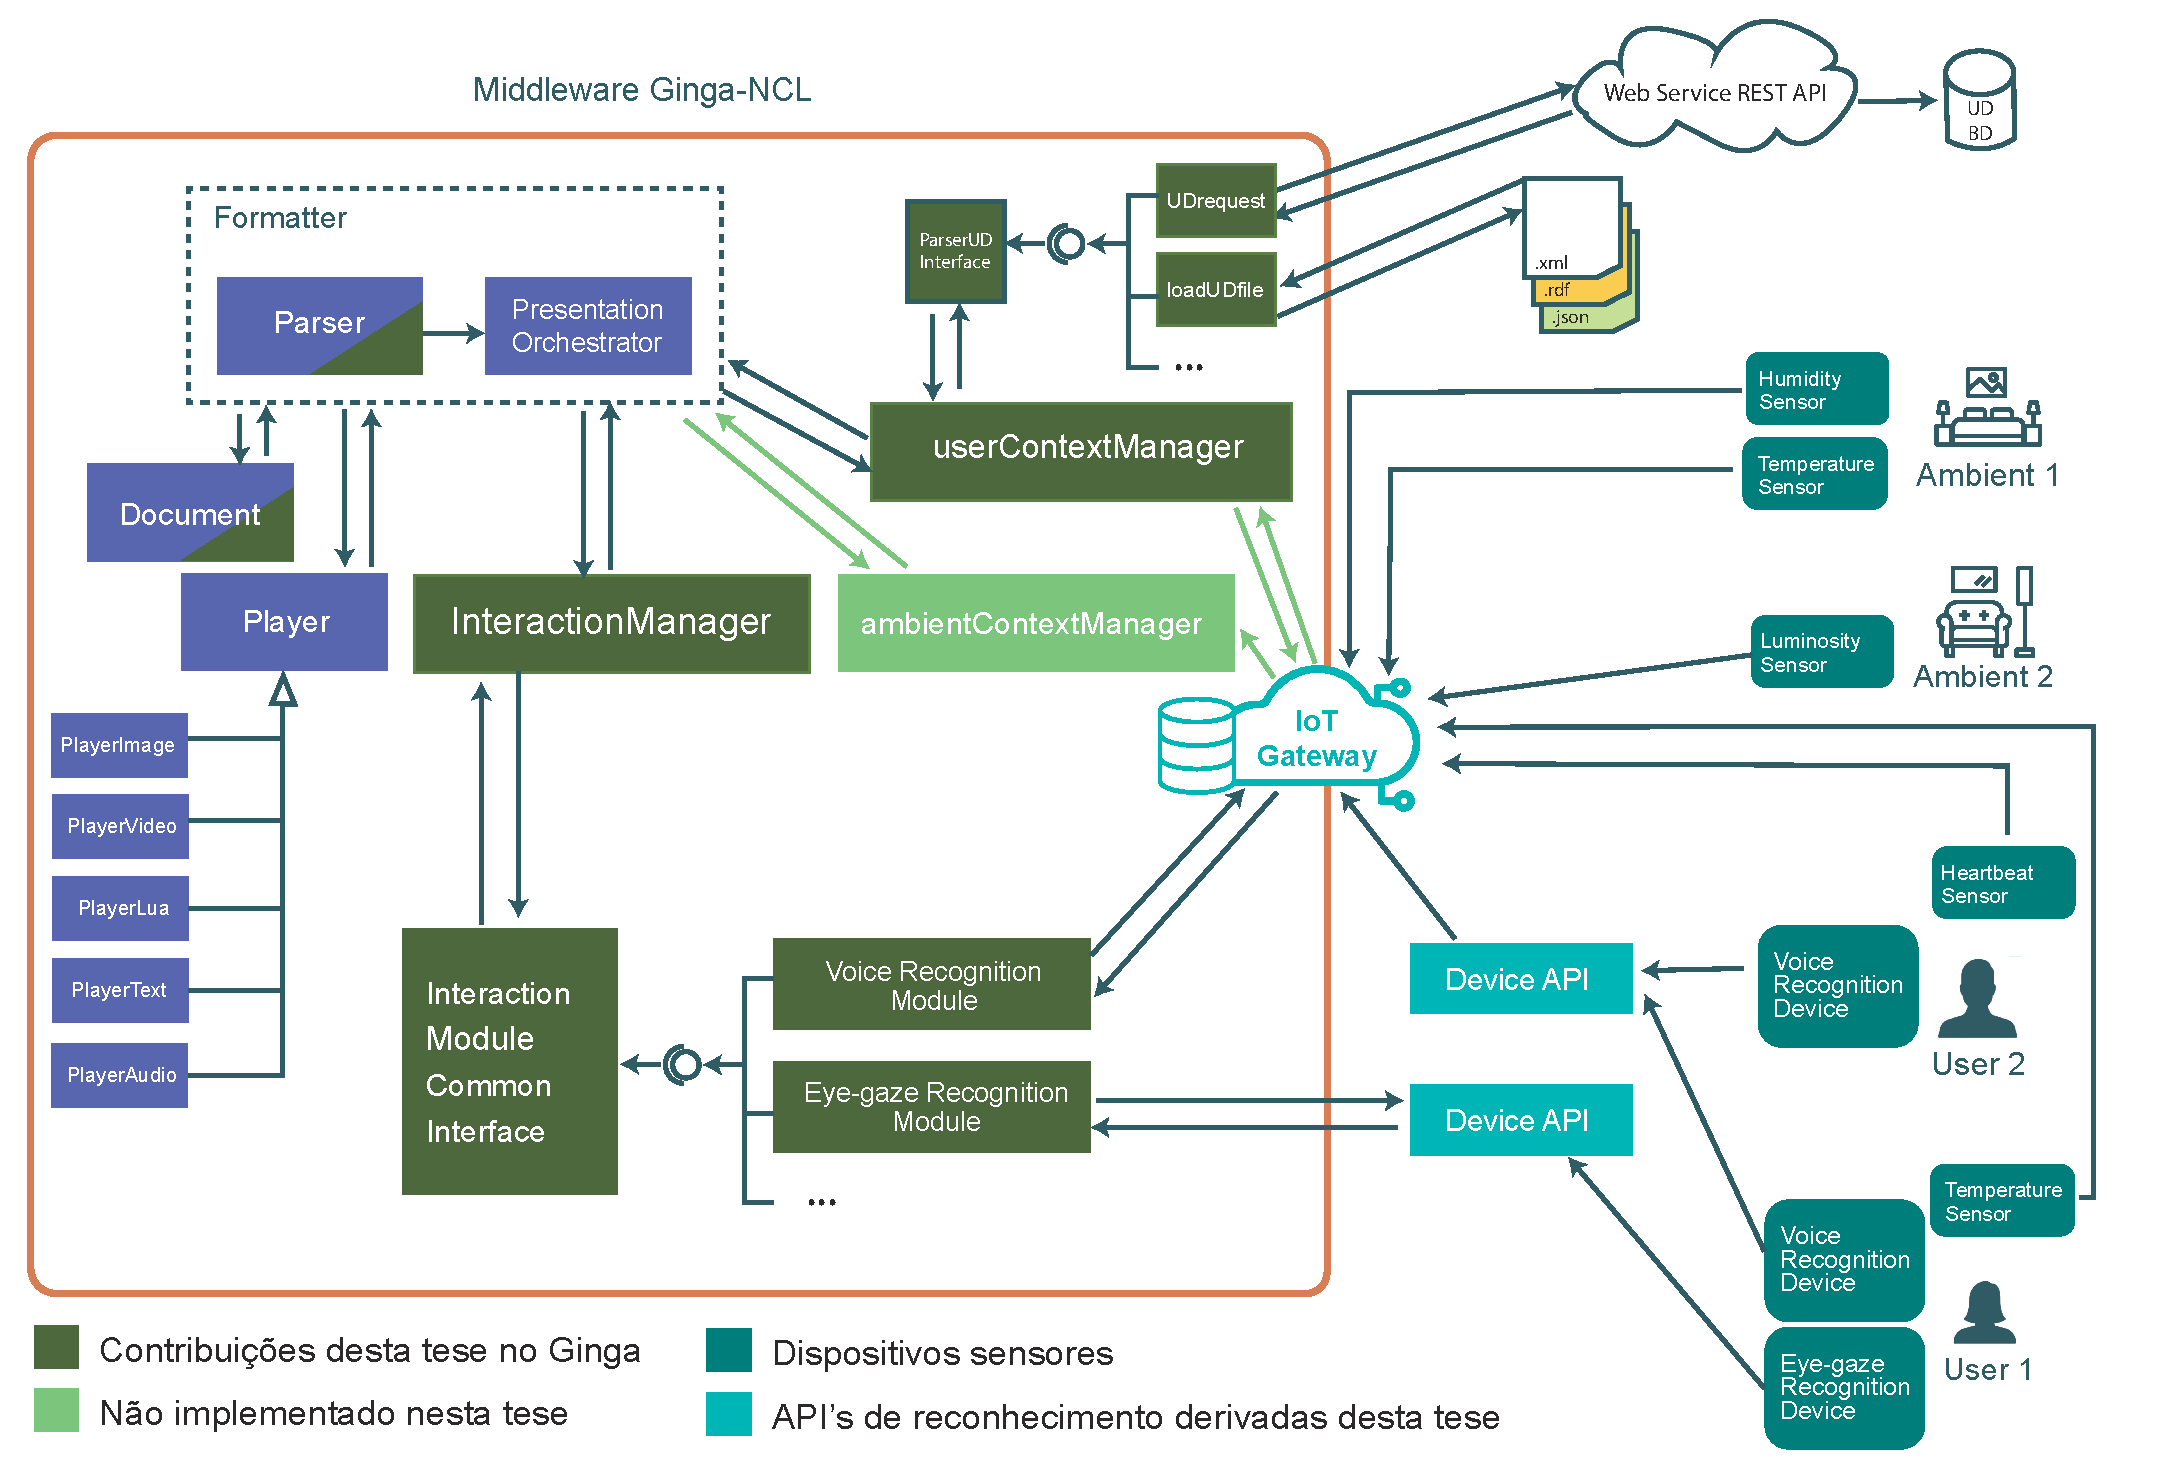
\includegraphics[scale=0.43, keepaspectratio=true]{figuras/ArqPropExt.pdf}
    \caption{Arquitetura estendida do Ginga-NCL para suporte à interação multimodal com múltiplos usuários.}
    \label{fig:arquitetura}
\end{figure}

\section{Interação multimodal e multiusuário}

O componente \textit{Formatter}, presente na atual versão do Ginga, é o responsável por controlar a apresentação dos objetos de mídia que compõem uma aplicação. Além disso, este elemento manipula os eventos de interação do usuário com a aplicação. Ao iniciar uma aplicação multimídia, o \textit{Formatter} envia o documento NCL para o \textit{Parser}, que extrai as informações sobre os elementos que compõem a aplicação e as relações de sincronização espaço-temporal definidas pelo autor da aplicação multimídia. 

O controle das interações do usuário com a aplicação multimídia é realizado pelo componente \textit{InteractionManager} proposto neste trabalho. É por meio do \textit{InteractionManager} que os dispositivos de interação se comunicam com o \textit{Formatter}, notificando-o quando ocorre uma interação por parte do usuário. O \textit{InteractionManager} ativa os diferentes módulos de interação, conforme especificado pelo documento NCL, e passa, para cada um deles, as informações sobre o que deve ser monitorado durante a execução da aplicação. A fim de permitir que a implementação seja facilmente estendida para adição de novas modalidades de interação, foi criada uma interface (\textit{Interaction Module Common Interface}), que deve ser implementada por cada módulo de interação específico. Note que, se a aplicação não utiliza um determinado tipo de interação, o módulo correspondente não será iniciado pelo \textit{InteractionManager} desnecessariamente.

Para a implementação da interação multimodal proposta nesta tese, os componentes \textit{Parser} e \textit{Formatter} foram estendidos, para dar suporte ao reconhecimento de novos tipos de eventos definidos em NCL 4.0 e  detalhados no Capítulo~\ref{cap:cap4}. Se elos da aplicação NCL associam eventos de interação a usuários ou perfis específicos, na fase de análise do documento, o \textit{Parser} faz o mapeamento entre a interação e o usuário associado a ela, por meio da análise dos elementos \textit{<link>} especificados. Por exemplo, ao analisar o elo definido na Listagem \ref{lst:ncl_multmodal}, o \textit{Parser} irá informar ao \textit{Formatter} que é preciso ativar o módulo responsável pelo reconhecimento de voz~(\textit{Voice Recognition Module}), além de enviar para esse módulo o usuário "\textit{user1}" (atributo \textit{user}) e palavra chave  "\textit{play}" (atributo \textit{key}) relacionados à interação e que ele deve notificar ao reconhecedor. Essa notificação é feita ao módulo \textit{InteractionManager}.

\begin{lstlisting}[language=ncl,label=lst:ncl_multmodal, caption={Conector e elo para interação mutimodal em NCL estendido}]

...
<connectorBase>
   <causalConnector id="onVoiceRecognitionStart">
      <connectorParam name="key"/>
      <connectorParam name="user"/>      
      <simpleCondition role="onVoiceRecognition" key="$\$$key" user= "$\$$user"/>
      <simpleAction role="start" />
   </causalConnector>  
</connectorBase>
...
<link xconnector="onVoiceRecognitionStart">
 	<bind role="onVoiceRecognition" component="botanicalGardenImage">
  		<bindParam name="key" value="play"/>
   		<bindParam name="user" value="user1"/>
 	</bind>
 	<bind role="start" component="botanicalGardenVideo"/>
 </link> 
...
\end{lstlisting}

%O controle das interações do usuário com a aplicação multimídia é realizado pelo componente \textit{InteractionManager} proposto neste trabalho. É por meio do \textit{InteractionManager} que os dispositivos de interação se comunicam com o \textit{Formatter}, notificando-o quando ocorre uma interação por parte do usuário. O \textit{InteractionManager} ativa os diferentes módulos de interação, conforme especificado pelo documento NCL, e passa, para cada um deles, as informações sobre o que deve ser monitorado durante a execução da aplicação. A fim de permitir que a implementação seja facilmente estendida para adição de novas modalidades de interação, foi criada uma interface (\textit{Interaction Module Common Interface}), que deve ser implementada por cada módulo de interação específico. Note que, se a aplicação não utiliza um determinado tipo de interação, o módulo correspondente não será iniciado pelo \textit{InteractionManager} desnecessariamente.

Os módulos de interação e o \textit{InteractionManager} se comunicam através de métodos pré-definidos pela interface (\textit{Interaction Module Common Interface}). Por exemplo, o \textit{InteractionManager}, ao ativar um módulo de interação, envia um objeto JSON (\textit{JavaScript Object Notation}) com uma lista de \textit{keys} que devem ser monitoradas pelo módulo, e os usuários relacionados àquela interação. Esta lista de \textit{keys} enviada pelo \textit{InteractionManager} depende do tipo de interação. Por exemplo, para o \textit{Voice Recognition Module}, são enviadas palavras ou frases a serem reconhecidas, e para o \textit{Gesture Recognition Module}, os tipos de gestos utilizados na aplicação. A Listagem~\ref{lst:json-exemplo} mostra um exemplo de JSON que segue o modelo para mapeamento de reconhecimento de voz, que gera o evento definido no \textit{link} na Listagem~\ref{lst:ncl_multmodal}.

\begin{lstlisting}[language=ncl,label=lst:json-exemplo, caption={Exemplo de JSON que usa o modelo para mapeamento de reconhecimento de voz para a Listagem~\ref{lst:ncl_multmodal}.}]
 {
    "userKeyList": [
        {
            "user": "user1",
            "key": [ "play"]
        }
    ]
 }
\end{lstlisting}



Na arquitetura proposta ilustrada na Figura \ref{fig:arquitetura}, pode-se perceber que o trabalho de reconhecimento da interação não é feito pelo formatador, evitando assim uma sobrecarga de processamento. Ele é notificado pelo \textit{InteractionManager} apenas se ocorrer uma interação que deve ser tratada pela aplicação. Ou seja, em uma aplicação multimídia que especifica apenas interação por voz, tendo como \textit{key} a palavra "\textit{play}", caso o usuário diga quaisquer outras palavras diferentes, nenhuma notificação será enviada ao \textit{InteractionManager}, e consequentemente ao formatador. Além disso, quando um módulo de interação específico notifica uma interação, ele pode também informar qual o usuário que a realizou, que no exemplo seria o "user1". Dentre os métodos que os módulos de interação devem implementar estão: \textit{start()}, \textit{setUserKeyList(json)} e \textit{stop()}, que possibilita ao \textit{InteractionManager} iniciar, passar as informações (\textit{keys}) que devem ser reconhecidas e parar o módulo de interação. Estes métodos são virtuais na classe \textit{InteractionModule}, portanto para desenvolver um novo módulo de interação funcionando nesta arquitetura, é necessário estender a classe \textit{InteractionModule}. Exemplos de subclasses de \textit{InteractionModule} na Figura \ref{fig:arquitetura} são \textit{Eye-gaze Recognition Module} e \textit{Voice Recognition Module}. 

\subsection{Reconhecimento de Voz em Ginga-NCL}

Com objetivo de validar a solução proposta, esta seção apresenta a implementação do módulo \textit{VoiceRecognitionModule} no Ginga-NCL utilizando uma API de reconhecimento de voz. A implementação de \textit{VoiceRecognitionModule} no Ginga utiliza a interface de comunicação comum a todos os dispositivos de interação (\textit{Interaction Module Common Interface}). Nesta implementação, o dispositivo de reconhecimento de voz se comunica com o Ginga utilizando o protocolo MQTT \cite{hunkeler2008mqtt}. Para isso, foram usadas funções do \textit{Google Cloud} para suprir a necessidade da conversão \textit{speech-to-text} \cite{bijl2001speech}. Inicialmente, é necessária a aplicação \textit{Google Assistant} para captar a voz do usuário e uma \textit{Action} do Google. Uma \textit{Action} é, essencialmente, uma aplicação que roda sobre o \textit{Google Assistant}, estendendo suas funcionalidades. Como ilustrado pela Figura~\ref{fig:action}, para a \textit{Action} se comunicar com o broker MQTT, ela utiliza o serviço Google \textit{Firebase} para que seja feita a publicação MQTT. 

Em resumo, o \textit{VoiceRecognitionModule} se inscreve em um tópico MQTT criado para o módulo de reconhecimento de voz. Isso é feito na execução do método \textit{start()} e portanto a instância passa a ouvir publicações no tópico que a \textit{Action} usa. Assim, a API do Google publica uma mensagem nesse tópico, significando que o dispositivo reconheceu o que foi dito. Quando ocorre a publicação do texto reconhecido no broker MQTT, o \textit{VoiceRecognitionModule} compara seu conteúdo com a lista de \textit{keys} e \textit{users} de interesse da aplicação. Se for uma palavra ou frase associado a um usuário de interesse ao Ginga, notifica o \texttt{InteractionManager}, que por sua vez dispara o evento de reconhecimento de voz no formatador.

\begin{figure}[h!]
    \centering
    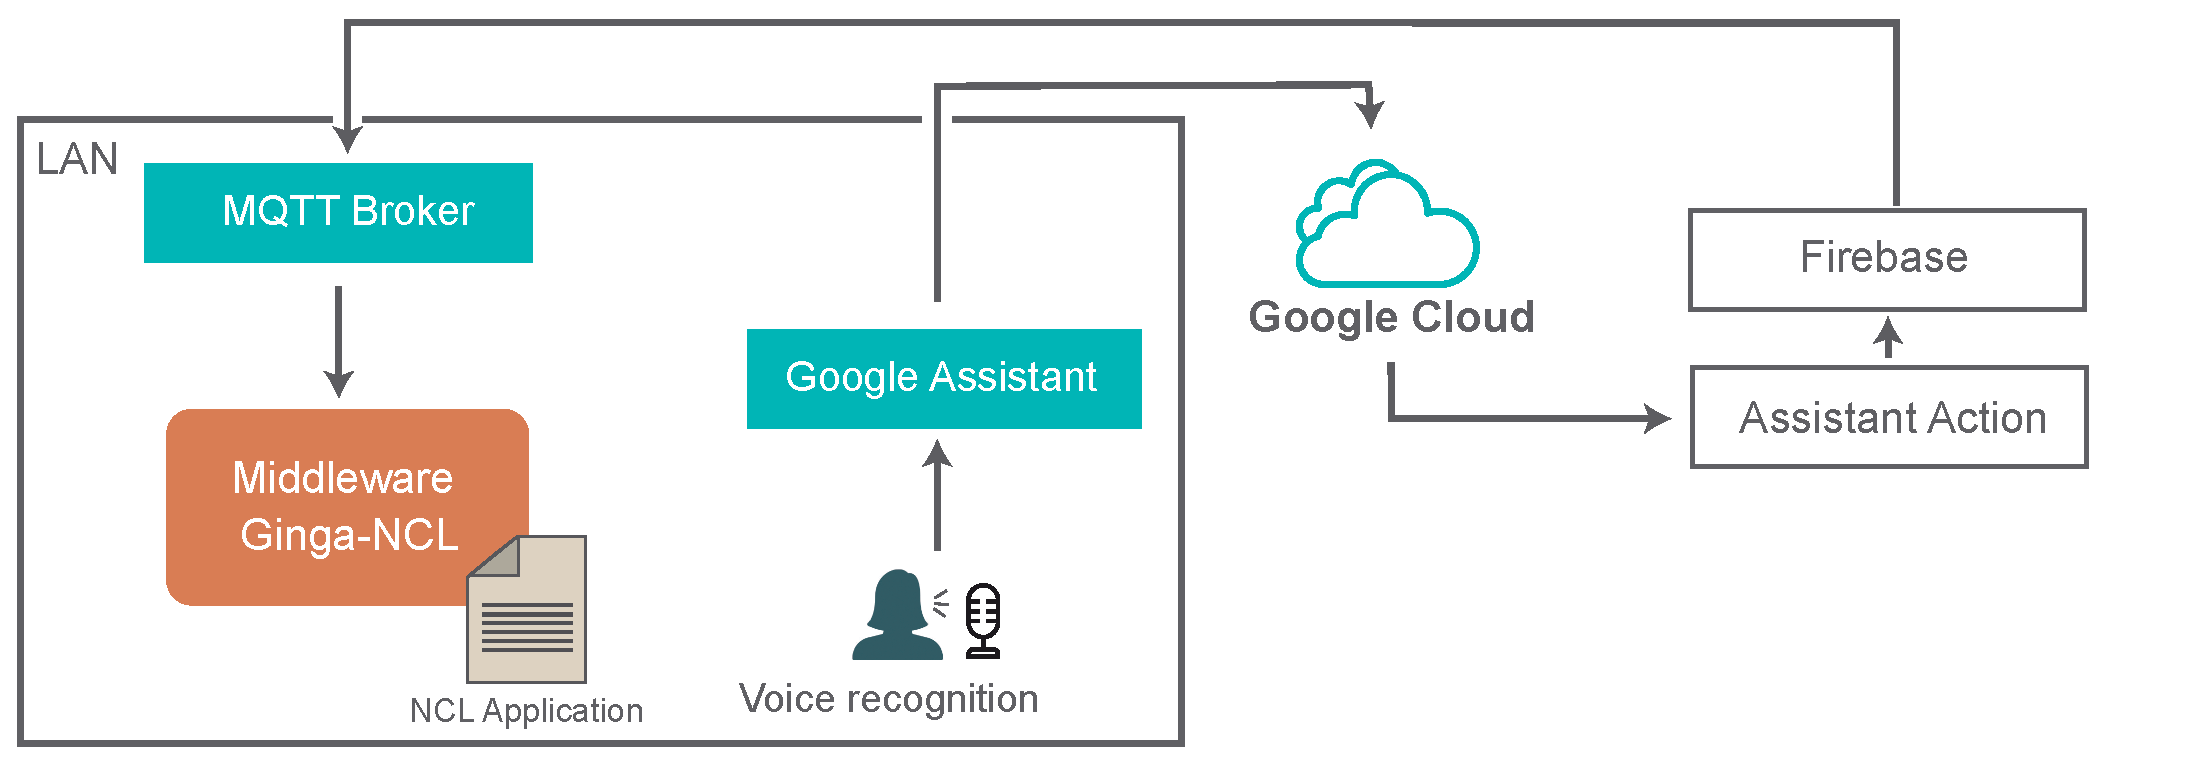
\includegraphics[scale=0.35, keepaspectratio=true]{figuras/arq-action-eng.pdf}
    \caption{Arquitetura do reconhecimento de voz na implementação atual.}
    \label{fig:action}
\end{figure}

A \textit{Action}, ao ser invocada, encaminha em forma de texto, todos comandos de voz que sejam precedidos por "TV". Desse modo, caso se queira executar na aplicação um comando denominado "iniciar", diz-se "TV iniciar". Há, ainda, uma configuração opcional de perfis de usuário. Ao dizer "Definir perfil como...", o que vier depois é vinculado ao dispositivo corrente como sendo o perfil ou a identificação daquele usuário. Feito isso, todos os comandos enviados à aplicação são precedidos por esse perfil ou identificação, relacionado ao usuário que interagiu.

A título de exemplo, em uma aplicação que contém um terapeuta e um paciente, de forma que cada perfil tem acesso a um conjunto de comandos diferentes, o usuário ao se identificar por terapeuta, em seu dispositivo, invoca "Definir perfil como terapeuta" e, analogamente, o paciente faz o mesmo. A partir disso, a aplicação será capaz de decidir, baseado nos perfis, quem invoca qual comando.

Outra implementação, seguindo a arquitetura da Figura~\ref{fig:arquitetura}, foi proposta em \cite{montevecchi2020providing}, onde sensores de rastreamento ocular permitem que os usuários interajam pelo olhar com aplicativos multimídia, proporcionando assim também uma nova modalidade de interação para as aplicações de TV digital. Em \cite{montevecchi2020providing}, foi proposta uma extensão Ginga-NCL para fornecer interação através de fixação do olhar usando um dispositivo rastreador de olhos e permitir o uso de um novo tipo de evento para autoria  em NCL, chamado \textit{EyeGaze}.

O trabalho de  \cite{valentim2020possibilitando} utiliza a  arquitetura proposta na Figura~\ref{fig:arquitetura} para possibilitar o reconhecimento de expressões faciais para que a TV que seja agnóstica à implementação do algoritmo de reconhecimento. Como prova de conceito, a  proposta do artigo foi desenvolvida sob o \textit{middleware} Ginga-NCL. Foram realizadas duas implementações: a primeira baseada na versão atual do \textit{middleware} Ginga e a segunda baseada em uma extensão proposta ao \textit{middleware}, mostrando a viabilidade da proposta apresentada.

\section{Suporte Multiusuário e Informações de Contexto}

A atual versão do \textit{middleware} Ginga-NCL captura as interações vindas de dispositivos como controle remoto, mouse ou teclado representando a interação de um usuário somente. Suas informações são armazenadas em um nó de conteúdo do tipo \textit{settingsNode} onde também são armazenadas informações gerais da aplicação NCL. Só é permitido um nó desse tipo por aplicação NCL. Algumas dessas propriedades não podem ser alteradas durante a execução da aplicação. Se mais de um usuário interage com a aplicação e essa precisa mudar seu comportamento de acordo com propriedades específicas de quem participa da experiência, não seria possível construir um documento NCL para atender a esse caso de uso na versão atual do Ginga-NCL.

O elemento XML <\textit{userAgent}> foi implementado por meio de uma estrutura \textit{user} que armazena propriedades de um usuário como um identificador e o caminho do arquivo onde estão suas informações individuais. Já o <\textit{userProfile}> foi implementado com a construção da estrutura \textit{profile} que mantém um identificador, numero mínimo e máximo de usuários que podem estar associados ao perfil e o caminho para as informações do perfil. A implementação mantém, no formatador, uma lista de estruturas do tipo \textit{user} e outra lista do tipo \textit{profile}. Desta forma, é possível ao formatador associar os \textit{links} de interação com os usuários ou perfis a estas listas; Carregar informações destes usuários para nós de conteúdo do tipo \textit{userSettingsNode} podendo também criar elos com esses nós. Finalmente pode-se associar a essa lista sensores, que podem coletar informações dos usuários participantes da experiência multimídia, como batimento cardíaco ou temperatura.

Os elos são associados ao usuário da maneira como foi descrita na Seção anterior, ou seja, o \textit{InteractionManager} envia para os módulos as listas de usuário que participam dos elos por meio de seu atributo \textit{user}. O valor do atributo \textit{user} deve fazer parte das listas de \textit{users} ou \textit{profiles} mantidas pelo formatador. Assim o autor da aplicação precisa definir o elemento  \textit{userAgent} e/ou \textit{userProfile} para poder referenciá-lo em elos com eventos de interação.

Conforme apresentado na Figura~\ref{fig:arquitetura}, o \textit{userContextManager} gerencia a importação das informações associadas tanto a \textit{userAgent} quanto a \textit{userProfile}. As informações podem estar dispostas em arquivos como por exemplo XML, RDF ou JSON ou ainda estarem disponíveis em um banco de dados remoto  acessado por meio de API REST. O caminho do arquivo ou a string de conexão fica armazenada no atributo \textit{src} do \textit{userAgent} ou \textit{userProfile}. O carregamento dessas informações é feito por um módulo que implementa a interface \textit{ParserUDInterface}, como por exemplo, \textit{UDRequest} e \textit{loadUDFile}. Este módulo irá carregar todas as informações presentes no arquivo ou no banco de dados de acordo com a fonte de cada um. Para que um novo formato de arquivo seja contemplado pelo \textit{userContextManager}, basta implementar um classe filha de \textit{ParserUDInterface}. O módulo \textit{userContextManager} irá passar aos "importadores" (módulos que implementam \textit{ParserUDInterface}) todos os dados necessários para importação e armazenamento das propriedades desses usuários ou perfis. 

As informações trazidas serão armazenadas em nós de conteúdo do tipo \textit{userSettingsNode} gerenciados pelo \textit{UserContextManager}. Esses nós são instâncias de \textit{userSettingsNode} associados aos elementos  <\textit{userAgent}> ou <\textit{userProfile}>. Como prova de conceito, foi desenvolvido o módulo \textit{loadUDFile} para  arquivos XML seguindo o padrão MPEG-21 parte 22. Este módulo vai preencher o objeto da classe \textit{UserSettingsNode} associado a instância do \textit{UserAgent} respectivo.  Se o \textit{UserAgent} estiver associado ao \textit{UserProfile}, além das informações individuais referenciadas no \textit{UserAgent}, também serão consideradas as informações associadas aos \textit{UserProfiles}. A partir do momento em que as informações estão em nós do tipo \textit{userSettingsNode}, poderão ser utilizadas em elos com eventos de atribuição NCL.

As instâncias de \textit{UserSettingsNode} podem ser usadas também para armazenar informações lidas de um sensor em um ambiente IoT. Como pode-se verificar na Figura~\ref{fig:arquitetura}, pode-se ter sensores (com por exemplo \textit{Heartbeat Sensor} no User2) publicando leituras em um servidor IoT e o \textit{userContextManager} pode ler essas publicações e atualizar os nós do tipo \textit{UserSettingsNode} respectivos. Para isso, o gerenciador de contexto deve ter um assinante de um tópico no servidor IoT. Tomando como exemplo a arquitetura MQTT, pode-se ter um \textit{broker} MQTT recebendo publicações dos sensores e o gerenciador de contexto pode se inscrever nos mesmos tópicos de publicações dos sensores e atualizar as propriedades respectivas nos nós de conteúdo do tipo \textit{userSettingsNode} a partir da atualização das propriedades. Elos poderão ser ativados mudando o comportamento da aplicação de acordo com leituras feitas pelos sensores. De maneira análoga, o mesmo pode ser feito com sensores de ambiente (como por exemplo \textit{LuminositySensor} no Ambient 2 na Figura~\ref{fig:arquitetura}), publicando suas leituras no servidor IoT. E o gerenciador de contexto de ambientes (\textit{ambientContextManager}) pode pegar essas informações e atualizar os nós do tipo \textit{ambientSettingsNode}. Como também são nós de conteúdo, a atualização de suas propriedades pode ativar elos e disparar ações na aplicação. A implementação do \textit{ambientContextManager} 
é trabalho futuro.

Além de ler as informações publicadas pelos sensores de um servidor IoT, O \textit{userContextManager} pode também publicar informações específicas para que o dispositivo IoT leia, como por exemplo, informações para calibragem do dispositivo. Assim o gerenciador pode-se comunicar com o servidor nos dois sentidos. A comunicação entre o \textit{userContextManager} e o servidor IoT também 
é trabalho futuro.

Falta ressaltar que a arquitetura é extensível a vários tipos de evento de interação, dispositivos e sensores.

Este capítulo apresentou a implementação da proposta desta tese no \textit{middleware} Ginga-NCL, incluindo uma arquitetura extensível seus módulos e funcionamento geral. O capítulo exemplificou aplicações NCL desenvolvidas e utilizadas nos testes de funcionalidades. Apresentou também o formato dos dados que são trocados entre os módulos, como por exemplo, objetos JSON. O próximo capítulo apresenta a avaliação da proposta por meio de comparação com a implementação padrão atual do Ginga-NCL e também testes de carga que atestam o desempenho do \textit{middleware}.